\documentclass{beamer}
\usetheme{Antibes}

\usepackage{fontspec}
\usepackage[catalan]{babel}
\usepackage{hyperref}

\AtBeginSection[]
{
	\begin{frame}
		\frametitle{Contingut}
		\tableofcontents[currentsection]
	\end{frame}
}

\AtBeginSubsection[]
{
	\begin{frame}
		\frametitle{Contingut}
		\tableofcontents[currentsection,currentsubsection]
	\end{frame}
}

\title{Construcció d'una orquestra amb Raspberry Pi}
\author{Arnau Canyadell Miquel \and Joan Marcè Igual}

\begin{document}

\frame{\titlepage}
\section{Introducció}

\begin{frame}
	Crear amb Raspberry Pi una orquestra musical formada per un director i uns quants músics que interpreten el que els mana el director.
	\begin{figure}
		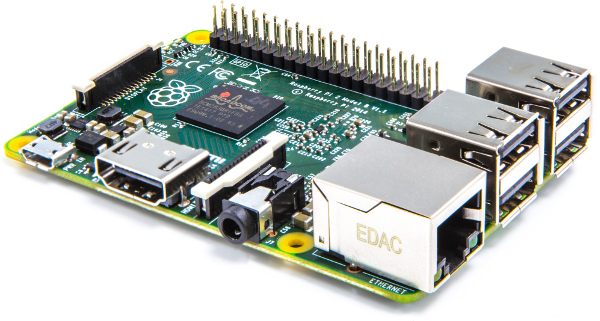
\includegraphics[width=0.475\linewidth]{images/raspberry}
		\hfill
		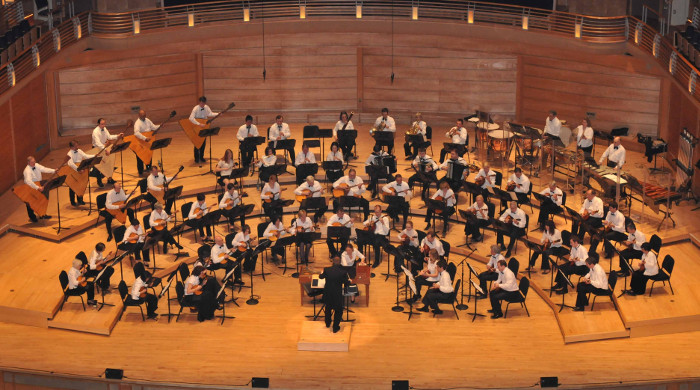
\includegraphics[width=0.475\linewidth]{images/orchestra}
	\end{figure}
\end{frame}

\section{Metodologia}

\begin{frame}
	\begin{itemize}[<+->]
		\item Repositori: \url{https://github.com/jmigual/projecte2}
		\item Trello amb objectius a curt i a llarg termini
		\item Llenguatge de programació: \texttt{Python}
	\end{itemize}
	\begin{figure}
		\hfill
		\includegraphics<1->[width=0.3\textwidth]{images/github}
		\hfill
		\includegraphics<2->[width=0.32\textwidth]{images/trello}
		\hfill
		\includegraphics<3->[width=0.3\textwidth]{images/python}
		\hfill
	\end{figure}
\end{frame}
\section{Feina feta}
\section{Objectius}
\section{Material}


\end{document}